\section{Objetivos y metodología de trabajo}
\label{sec:obj_metd}

En este capítulo se exponen los objetivos perseguidos con el desarrollo del presente Trabajo Fin de Máster, pasando por la infraestructura y tecnologías seleccionadas, y acabando con la metodología empleada para su ejecución. El trabajo se enmarca dentro del área del aprendizaje profundo, aplicados al problema de la predicción del flujo de tráfico urbano. El propósito es diseñar una solución capaz de anticipar el estado de la red viaria a corto plazo en la provincia de Bizkaia, utilizando datos abiertos y públicos de fuentes institucionales, lo cual permitirá evaluar tanto la capacidad de generalización de los modelos como su utilidad práctica en un contexto real. 

Como se analizó en el capítulo anterior, la predicción del tráfico urbano enfrenta importantes retos derivados de la alta variabilidad temporal y la compleja dependencia espacial de los datos. Entre los trabajos analizados, destaca el modelo Trafficformer de \cite{trafficformer}, que introduce un enfoque basado en Transformers mejorado mediante máscaras espaciales para filtrar ruido y enfocar la atención en interacciones relevantes entre nodos de la red. Aunque el modelo original fue diseñado para predecir velocidades de tráfico, su arquitectura resulta igualmente aplicable a la predicción de volúmenes de tráfico, esto es, la cantidad de vehículos que circulan por un punto dado en cada intervalo temporal, mediante una adaptación del preprocesamiento y del objetivo del modelo.

\subsection{Objetivos del proyecto}

El objetivo general de este Trabajo Fin de Máster es el diseño, implementación y evaluación de un sistema de predicción del tráfico urbano a corto plazo mediante el uso de técnicas de aprendizaje profundo, con especial énfasis en las redes neuronales de tipo Transformer. La solución desarrollada debe ser capaz de predecir con precisión el estado futuro del tráfico en diversos puntos de la red viaria de Bizkaia, aprovechando el valor añadido que ofrecen los datos abiertos procedentes de fuentes públicas, como los portales de Open Data del Gobierno Vasco. Para ello, se debe implementar y entrenar un modelo de predicción inspirado en el modelo Trafficformer, adaptado a volúmenes de tráfico. Este objetivo principal responde a la necesidad creciente de disponer de herramientas tecnológicas que permitan mejorar la gestión de la movilidad en entornos urbanos, facilitar la toma de decisiones estratégicas y operativas en tiempo real, y anticiparse a situaciones potenciales de congestión. La precisión de la predicción se configura como un factor clave en la eficacia de sistemas \acrshort{its} modernos, especialmente en contextos densamente poblados como el área metropolitana de Bilbao. 

Como primer objetivo específico se pretende analizar el conjunto de datos disponibles en el catálogo de datos abiertos del Gobierno Vasco ubicado en \cite{openDataGv}. Dentro del mismo, se pretende identificar y analizar el Api de tráfico de \cite{apiTraffic}, además de otros factores contextuales como la meteorología, que se ha demostrado influyente en la dinámica del tráfico y cuyo \acrshort{api} se ubica en \cite{apiMeteo}.

Asimismo, se plantea como segundo objetivo específico la validación empírica de los modelos mediante experimentación con datos reales, evaluando su rendimiento con métricas reconocidas en el ámbito de la predicción, tales como el error cuadrático medio o \acrshort{rmse}, el error absoluto medio o \acrshort{mae} o el error porcentual absoluto medio o \acrshort{mape}. La comparación entre distintos enfoques permitirá identificar las ventajas y limitaciones de cada uno, así como proponer mejoras que potencien su aplicabilidad.

Por último, se considera el tercer objetivo específico del trabajo ofrecer una reflexión crítica sobre el impacto potencial de este tipo de soluciones en el ámbito de la movilidad urbana y su eventual integración en sistemas de ayuda a la decisión de carácter público o privado. El valor añadido que se pretende aportar no reside únicamente en la capacidad predictiva del modelo, sino también en su posible contribución al desarrollo de una movilidad más eficiente, sostenible e inteligente.

\subsection{Infraestructura y tecnologías empleadas}

En este apartado se van a exponer todos los recursos seleccionados que van a servir de soporte para la consecución de los objetivos y el desarrollo del proyecto.

Para ello, se va a utilizar una infraestructura híbrida compuesta por recursos locales y servicios en la nube.
Como equipo de desarrollo se va a seleccionar el equipo personal, que se compone por un procesador Intel Core i7-10700K de 10ª generación desbloqueado, con 32 GB de memoria \acrshort{ram} DDR4, haciendo uso de 2 discos \acrshort{ssd} NVMe (512 GB + 1 TB) y un HDD de 2 TB como almacenamiento, equipado con una GPU Nvidia GTX 1070 con soporte CUDA y corriendo el Sistema Operativo Windows 11 Pro.

Este equipo permitirá realizar tareas de programación, experimentación y entrenamiento preliminar, si bien se anticipa que no será suficiente para entrenar modelos de gran tamaño o con grandes cantidades de datos.

Por ello, se deberá emplear una infraestructura remota para realizar los distintos entrenamientos. Dada la necesidad de cómputo intensivo, se contempla el uso de una instancia EC2 en Amazon Web Services (AWS), con una AMI optimizada para entrenamiento de modelos con PyTorch (por ejemplo, la AMI de Deep Learning de AWS con soporte GPU Tesla T4 o V100). Esta infraestructura permitirá acelerar significativamente el proceso de entrenamiento y validación.

Asimismo, se va a hacer uso de un servidor doméstico con \href{https://www.truenas.com/}{TrueNAS} Scale Electric Eel como sistema operativo, equipado con un procesador Intel Core i5-7400 de 7ª generación, con 16 GB de RAM DDR4 y dos discos duros de 4 TB configurados en RAID 1. Este servidor albergará una base de datos \href{https://www.mongodb.com/}{MongoDB} para almacenamiento estructurado de datos y \href{https://min.io/}{MinIO} como sistema de almacenamiento tipo S3, útil para almacenamiento masivo y backups. Todos esos servicios van a funcionar como contenedores \href{https://www.docker.com/}{Docker}.

En cuanto al software, se van a seleccionar los lenguajes de programación \href{https://kotlinlang.org/}{Kotlin} (con \href{https://gradle.org/}{Gradle} como herramienta de construcción) y \href{https://www.python.org/}{Python} (con \href{https://python-poetry.org/}{Poetry} como gestor de dependencias y de empaquetamiento). En cuanto a los entornos de desarrollo, se ha decidido hacer uso de la suite de Jetbrains, puesto que facilitan licencias para estudiantes y son muy completas (ofreciendo muchas funcionalidades y asistentes que hacen más productiva tu jornada). Estos IDE son \href{https://www.jetbrains.com/es-es/idea/}{IntelliJ IDEA} (para el desarrollo con Kotlin) y \href{https://www.jetbrains.com/es-es/pycharm/}{PyCharm} (para el desarrollo con Python). Para el control de versiones se va a emplear \href{https://git-scm.com/}{Git}, con repositorios en GitHub o GitLab.

Para el desarrollo del modelo de predicción de tráfico se ha optado por utilizar \href{https://pytorch.org/}{PyTorch} como backend principal. Esta decisión se fundamenta en la flexibilidad que ofrece esta biblioteca para la implementación de arquitecturas avanzadas, como redes neuronales recurrentes (LSTM, GRU), redes convolucionales (CNN), Graph Attention Networks (GAT) y modelos basados en Transformers. Además, PyTorch cuenta con una comunidad investigadora muy activa y un ecosistema maduro que incluye librerías especializadas como PyTorch Geometric o HuggingFace Transformers, altamente relevantes para el ámbito de este trabajo. A diferencia de otros entornos como TensorFlow/Keras, que destacan por su facilidad de uso en fases de prototipado, PyTorch ofrece un control más explícito sobre el flujo de datos y la personalización del entrenamiento, lo que resulta especialmente valioso en proyectos que requieren ajustar arquitecturas de manera específica para capturar correlaciones espaciotemporales complejas en el tráfico urbano. 

Estas decisiones se ven respaldadas por análisis comparativos recientes, como el realizado por DataCamp, donde se destaca que \textit{PyTorch} suele ser más rápido y proporciona mejores capacidades de depuración que \textit{Keras}. Estas características lo hacen especialmente adecuado para entornos de investigación y desarrollo de modelos complejos cite{datacamp2023}.

Además, UnfoldAI ofrece un análisis detallado sobre las fortalezas y debilidades de los principales frameworks de aprendizaje profundo. En su estudio comparativo se destaca que \textit{PyTorch} proporciona una mayor flexibilidad y control, lo que lo convierte en la opción preferida en entornos de investigación, mientras que \textit{Keras} sobresale por su simplicidad y facilidad de uso, resultando ideal para usuarios principiantes y tareas de prototipado rápido \cite{unfoldai2024}.

\subsection{Metodología de trabajo}

Para la consecución de los objetivos, tomando como referencia la solución Trafficformer, se ha pensado en estructurar el proyecto siguiendo un flujo de trabajo organizado en varias fases clave.

\begin{figure}[H]
	\centering
	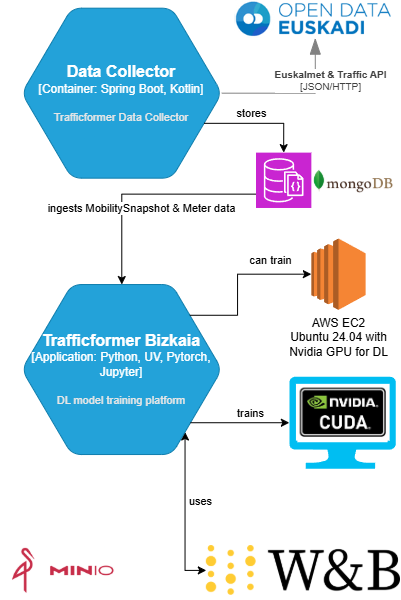
\includegraphics[width=0.6\textwidth]{includes/cap4/trafficformer_arch.png}
	\caption{Diagrama de arquitectura y pipeline general del proyecto.}
	\label{fig:pipeline-general}
\end{figure}

Este esquema proporciona una visión clara y sintetizada del flujo de trabajo, facilitando la comprensión global y la replicabilidad de las metodologías empleadas a lo largo de todo el proceso de investigación y desarrollo llevado a cabo en este TFM.

A continuación, se detallan las principales fases y componentes metodológicos del proyecto:

\begin{itemize}
	\item Adquisición y preprocesamiento de datos.
	\begin{itemize}
		\item \textbf{Datos}: se utilizarán datos abiertos provenientes del portal Open Data de Euskadi, principalmente de sensores que registran el número de vehículos que atraviesan puntos específicos de la red viaria en intervalos regulares.
		\item \textbf{Preprocesamiento}: se realizará la agregación temporal si es necesario (por ejemplo, a intervalos de 5 minutos), imputación de valores perdidos, normalización y generación de ventanas deslizantes para construir las series históricas.
	\end{itemize}
	\item Arquitectura del modelo. La arquitectura seguirá los principios del modelo Trafficformer, la cual se puede apreciar en la figura \ref{fig:trafficformer}, con los siguientes componentes adaptados:
	\begin{itemize}
		\item \textbf{Extracción temporal}: un MLP de dos capas se encargará de extraer patrones no lineales de las series de volumen de vehículos por punto de control.
		\item \textbf{Máscara espacial}: se construirá una matriz de adyacencia basada en la topología de la red viaria, utilizando distancias reales o tiempos de viaje para definir relaciones de vecindad relevantes.
		\item \textbf{Codificador Transformer}: mediante multi-head attention, el modelo extrae relaciones espaciales entre nodos cercanos, permitiendo una representación contextualizada del tráfico.
		\item \textbf{Predicción}: se proyectan las representaciones espacio-temporales a una predicción del número de vehículos que circularán por cada punto de la red en el siguiente intervalo.
	\end{itemize}
	\item Entrenamiento y evaluación.
	\begin{itemize}
		\item \textbf{Métricas}: se utilizarán MAE, RMSE y MAPE para comparar la predicción de conteos de vehículos.
		\item \textbf{Modelos base}: se tendrá como referencia el modelo \acrshort{mlp} desarrollado anteriormente.
		\item \textbf{Validación}: se aplicará validación temporal (walk-forward) para simular condiciones reales de predicción.
	\end{itemize}
\end{itemize}

Como consecuencia, se prevé llevar a cabo las siguientes tareas.

\begin{itemize}
	\item Extracción y almacenamiento de datos. Desarrollo de un módulo en Kotlin para conectar con las \acrshort{api} públicas de tráfico y meteorología de Open Data Euskadi. Almacenamiento de los datos crudos en MongoDB y objetos binarios (imágenes, CSVs temporales) en MinIO.
	\item Preprocesamiento y transformación de datos. Conversión de datos crudos en estructuras listas para entrenamiento, mediante scripts en Python. Aplicación de técnicas de normalización, resampleo temporal y gestión de datos faltantes.
	\item Entrenamiento de modelos neuronales. Implementación de un modelo base \acrshort{mlp} para establecer una línea base de rendimiento. Posterior implementación de un modelo Transformer adaptado al tráfico, con atención espacio-temporal y uso de máscaras de conectividad vial.
	\item Evaluación comparativa. Evaluación de los modelos con un conjunto de métricas estándar (\acrshort{mae}, \acrshort{rmse}, \acrshort{mape}). Comparativa entre modelos para seleccionar el más adecuado para el caso de uso.
	\item Validación y conclusiones. Validación en escenarios reales y extracción de conclusiones sobre la utilidad del modelo. Estudio de la viabilidad de su aplicación en entornos reales, como el soporte a \acrshort{its} o planificación urbana.
\end{itemize}

\subsection{Fundamentos matemáticos del modelo Trafficformer}

Para aportar una visión rigurosa y formal del modelo propuesto, a continuación se detalla la formulación matemática de Trafficformer, describiendo sus componentes principales y la notación empleada a lo largo de este trabajo.

\subsubsection*{Componentes principales}

\paragraph*{1. Traffic Input.}  
El punto de partida del modelo es una matriz histórica de aforos:

\[
S_t^{I}\in\mathbb{R}^{N\times I},
\]

donde $N$ representa la longitud de la ventana temporal (número de pasos de tiempo considerados) e $I$ es el número de nodos o sensores de la red. Para cada nodo $i$, se recoge una secuencia temporal de sus últimas $N$ mediciones de aforos, lo que puede visualizarse como un tensor tiempo × nodo.

El modelo también emplea una máscara espacial, construida a partir de la distancia física y las relaciones topológicas entre nodos:

\[
M^{P}\in\mathbb{R}^{I\times I}.
\]

Se trata de una matriz binaria que determina qué pares de nodos pueden influirse mutuamente, filtrando las interacciones irrelevantes (por ejemplo, nodos distantes o no conectados directamente en la red viaria).

\paragraph*{2. Temporal Feature Extractor}  

Cada columna de $S_t^{I}$, correspondiente a la serie temporal de un nodo, se procesa mediante un \emph{Multi-Layer Perceptron} (MLP) compartido. El resultado es una matriz de embeddings temporales por nodo:

\[
S_t^{C1}\in\mathbb{R}^{I\times d_t}.
\]

\paragraph*{3. Traffic Node Feature Interaction}  

Las representaciones temporales se combinan a través de un mecanismo de \emph{Multi-head Self-Attention}, donde la máscara $M^{P}$ restringe la atención a los nodos vialmente conectados. La estructura sigue el esquema Transformer estándar: atención $\rightarrow$ \textsc{Add \& Norm} $\rightarrow$ Feed-Forward $\rightarrow$ \textsc{Add \& Norm}. El resultado es un embedding espaciotemporal enriquecido:

\[
Z_t\in\mathbb{R}^{I\times d_s}.
\]

\paragraph*{4. Traffic Capacity Forecasting}  

Finalmente, un segundo MLP por nodo transforma $Z_t$ en las predicciones para los siguientes $H$ pasos temporales:

\[
\hat{V}_{t+1:t+H}\in\mathbb{R}^{I\times H},
\]

donde $H$ es el horizonte de predicción.

\subsubsection*{Resumen y puntos clave}

La Figura~\ref{fig:trafficformer} muestra el flujo de información entre los diferentes módulos del modelo. A continuación, se sintetiza en una sola expresión el pipeline completo:

\[
S_t^{I}\;
\xrightarrow[\text{MLP}]{\text{Temporal}}\;
S_t^{C1}\;
\xrightarrow[\;M^{P}\;]{\text{Self-Attention}}\;
Z_t\;
\xrightarrow[\text{MLP}]{\text{Regresión}}\;
\hat{V}_{t+1:t+H}
\]

Para mayor claridad, en la Tabla~\ref{tab:simbolos_trafficformer} se resume la notación empleada en esta sección.
\begin{table}[H]
	\centering
	\small
	\caption{Notación de los principales símbolos utilizados en la formulación de Trafficformer.}
	\label{tab:simbolos_trafficformer}
	\begin{tabularx}{\textwidth}{@{}>{$}c<{$}X@{}}
		\toprule
		\textbf{Símbolo} & \textbf{Descripción} \\ 
		
		\midrule
		N & Longitud de la ventana histórica (nº de pasos de tiempo) \\[2pt]
		I & Número total de nodos/sensores en la red \\[2pt]
		S_t^{I} & Matriz de características históricas de tamaño $N\times I$ \\[2pt]
		M^{P} & Máscara espacial ($I\times I$) que pondera la atención entre nodos \\[2pt]
		S_t^{C1} & Embedding temporal por nodo ($I\times d_t$) \\[2pt]
		Z_t & Embedding espaciotemporal final ($I\times d_s$) \\[2pt]
		\hat{V}_{t+1:t+H} & Aforos predichos para los próximos $H$ pasos \\ 
		
		\bottomrule
	\end{tabularx}
\end{table}

Por último, se destacan a continuación varios aspectos clave del diseño de Trafficformer que justifican su elección y eficacia para la predicción de tráfico:

\begin{itemize}
	\item El modelo \emph{desacopla} el aprendizaje temporal del aprendizaje espacial.
	\item La máscara $M^{P}$ introduce conocimiento a priori de la topología vial, lo que acelera la convergencia y mejora la interpretabilidad.
	\item Los MLP son ligeros y comparten pesos entre nodos, reduciendo la complejidad frente a arquitecturas basadas en LSTM o CNN.
\end{itemize}

\vspace{0.5cm}

Esta formulación matemática resume de forma rigurosa el funcionamiento interno de Trafficformer y proporciona la base conceptual sobre la que se desarrolla y adapta el modelo en el presente trabajo.
